\chapter{Séries temporelles}

\begin{wrapfigure}{r}{3cm}
\Youtube{https://youtu.be/xrdCY4iN40s}
\end{wrapfigure}

Les capteurs virtuels que nous avons programmés jusqu’à présent émettent les données à chaque fois que celles-ci sont mesurées. Cela permet au serveur de suivre en temps réel le comportement du système étudié. Mais dans certains cas, le temps réel n’est pas nécessaire et il est préférable de limiter le nombre d’émissions, par exemple pour économiser l'énergie du capteur.

Pour ce faire, nous pouvons utiliser un tableau qui va accumuler les valeurs et l’envoyer quand le tableau atteint une certaine taille.


\section{Envoi d'un tableau}

Le programme \pprog{minimal\_humidity1.py} accumule les données dans un tableau \texttt{h\_humidity} quand celui-ci atteint 30 élements (ligne 17), les données sont envoyées au serveur.

\pythonlst{minimal\_humidity1.py}



\begin{termc}[backgroundcolor=\color{palerod}, language=json, basicstyle=\ttfamily\small, escapechar=#]
1 4 [3241]
2 7 [3241, 2945]
3 10 [3241, 2945, 2762]
4 13 [3241, 2945, 2762, 2625]
5 16 [3241, 2945, 2762, 2625, 2480]
6 19 [3241, 2945, 2762, 2625, 2480, 2769]
\end{termc}

Le premier chiffre de la ligne indique le nombre d'éléments et le second la taille dans le codage CBOR. On remarque que l'ajout d'un élément augmente la taille du tableau de 3 octets. Les valeurs correspondant à une mesure d'humidité ne varient pas fortement. Ainsi un tableau de 30 mesures a une taille de 92 octets.

\section{Codage par différence}

On peut optimiser le volume de données transférées en utilisant un codage par delta (i.e. la variation de l'humidité). La première valeur du tableau correspond à la valeur mesurée tandis que les suivantes représentent la différence entre la valeur mesurée et la précédente.

\pythonlst[firstline=17,lastline=26,  firstnumber=17]{minimal\_humidity2.py}%[firstline=282,lastline=19, firstnumber=282]

Le programme \pprog{minimal\_humidity2.py} gère différemment le remplissage du tableau~:

\begin{itemize}
    \item ligne 14 et 15, si le tableau est vide, le tableau est créé avec la valeur msesurée,
    \item ligne 16 à 22, sinon si le tableau est plein, il est sérialisé en CBOR et envoyé au serveur, puis réinitialisé avec la valeur mesurée,
    \iten ligne 23 et 24, sinon la différence entre la précédente valeur et celle mesurée est stockée dans le tableau.
\end{itemize}

       \vspace{1em}

Le listing suivant donne un exemple d'exécution.

\begin{termc}[backgroundcolor=\color{palerod}, language=json, basicstyle=\ttfamily\small, escapechar=#]
1 4 [2521]
2 6 [2521, 79]
3 8 [2521, 79, 224]
4 10 [2521, 79, 224, -40]
5 12 [2521, 79, 224, -40, -112]
6 13 [2521, 79, 224, -40, -112, 1]
7 15 [2521, 79, 224, -40, -112, 1, 130]
8 18 [2521, 79, 224, -40, -112, 1, 130, -288]
9 21 [2521, 79, 224, -40, -112, 1, 130, -288, 299]
\end{termc}

Ceci met en valeur deux souplesses de CBOR :
\begin{itemize}
    \item la taille du tableau est dynamique. Si l’on change le nombre de valeurs à transmettre, le tableau l’indique et l’on n’a pas besoin de modifier le code du récepteur ;
    \item la taille des données dépend de leur valeur. Pour les variations entre -24 et +23, un seul octet sera nécessaire. On le voit sur l’exemple précédent : l’ajout de la valeur '1' dans le tableau fait passer la taille de la représentation CBOR de 12 à135 octets. Les valeurs entre 256 et +255 sont transmises sur 2 octets ; il est donc possible de cette manière d’optimiser la transmission sans ajouter de contrainte. S’il y avait une brusque variation de l’humidité, la représentation CBOR s’adapterait pour la transmettre.
\end{itemize}

La taille est réduite d"un tiers (environ 66 octets) pour transmettre la même information.

\section{Architecture}

La figure~\vref{fig-client-serveur} représente l'architecture générale du système. Le programme \pprog{minimal\_humidity2.py} fournit les séries temporelles. Il reste à définir le programme serveur qui va les traiter et faire appel à un autre service pour les afficher sous forme de graphe. 

       \vspace{1em}


Si l'on suit le flux d'information, le capteur va produire des données au format CBOR pour être compact et le programme serveur va transformer cette information en une structure JSON respectant les spécifications du service d'affichage.

\begin{figure}[tbp]
\centerline{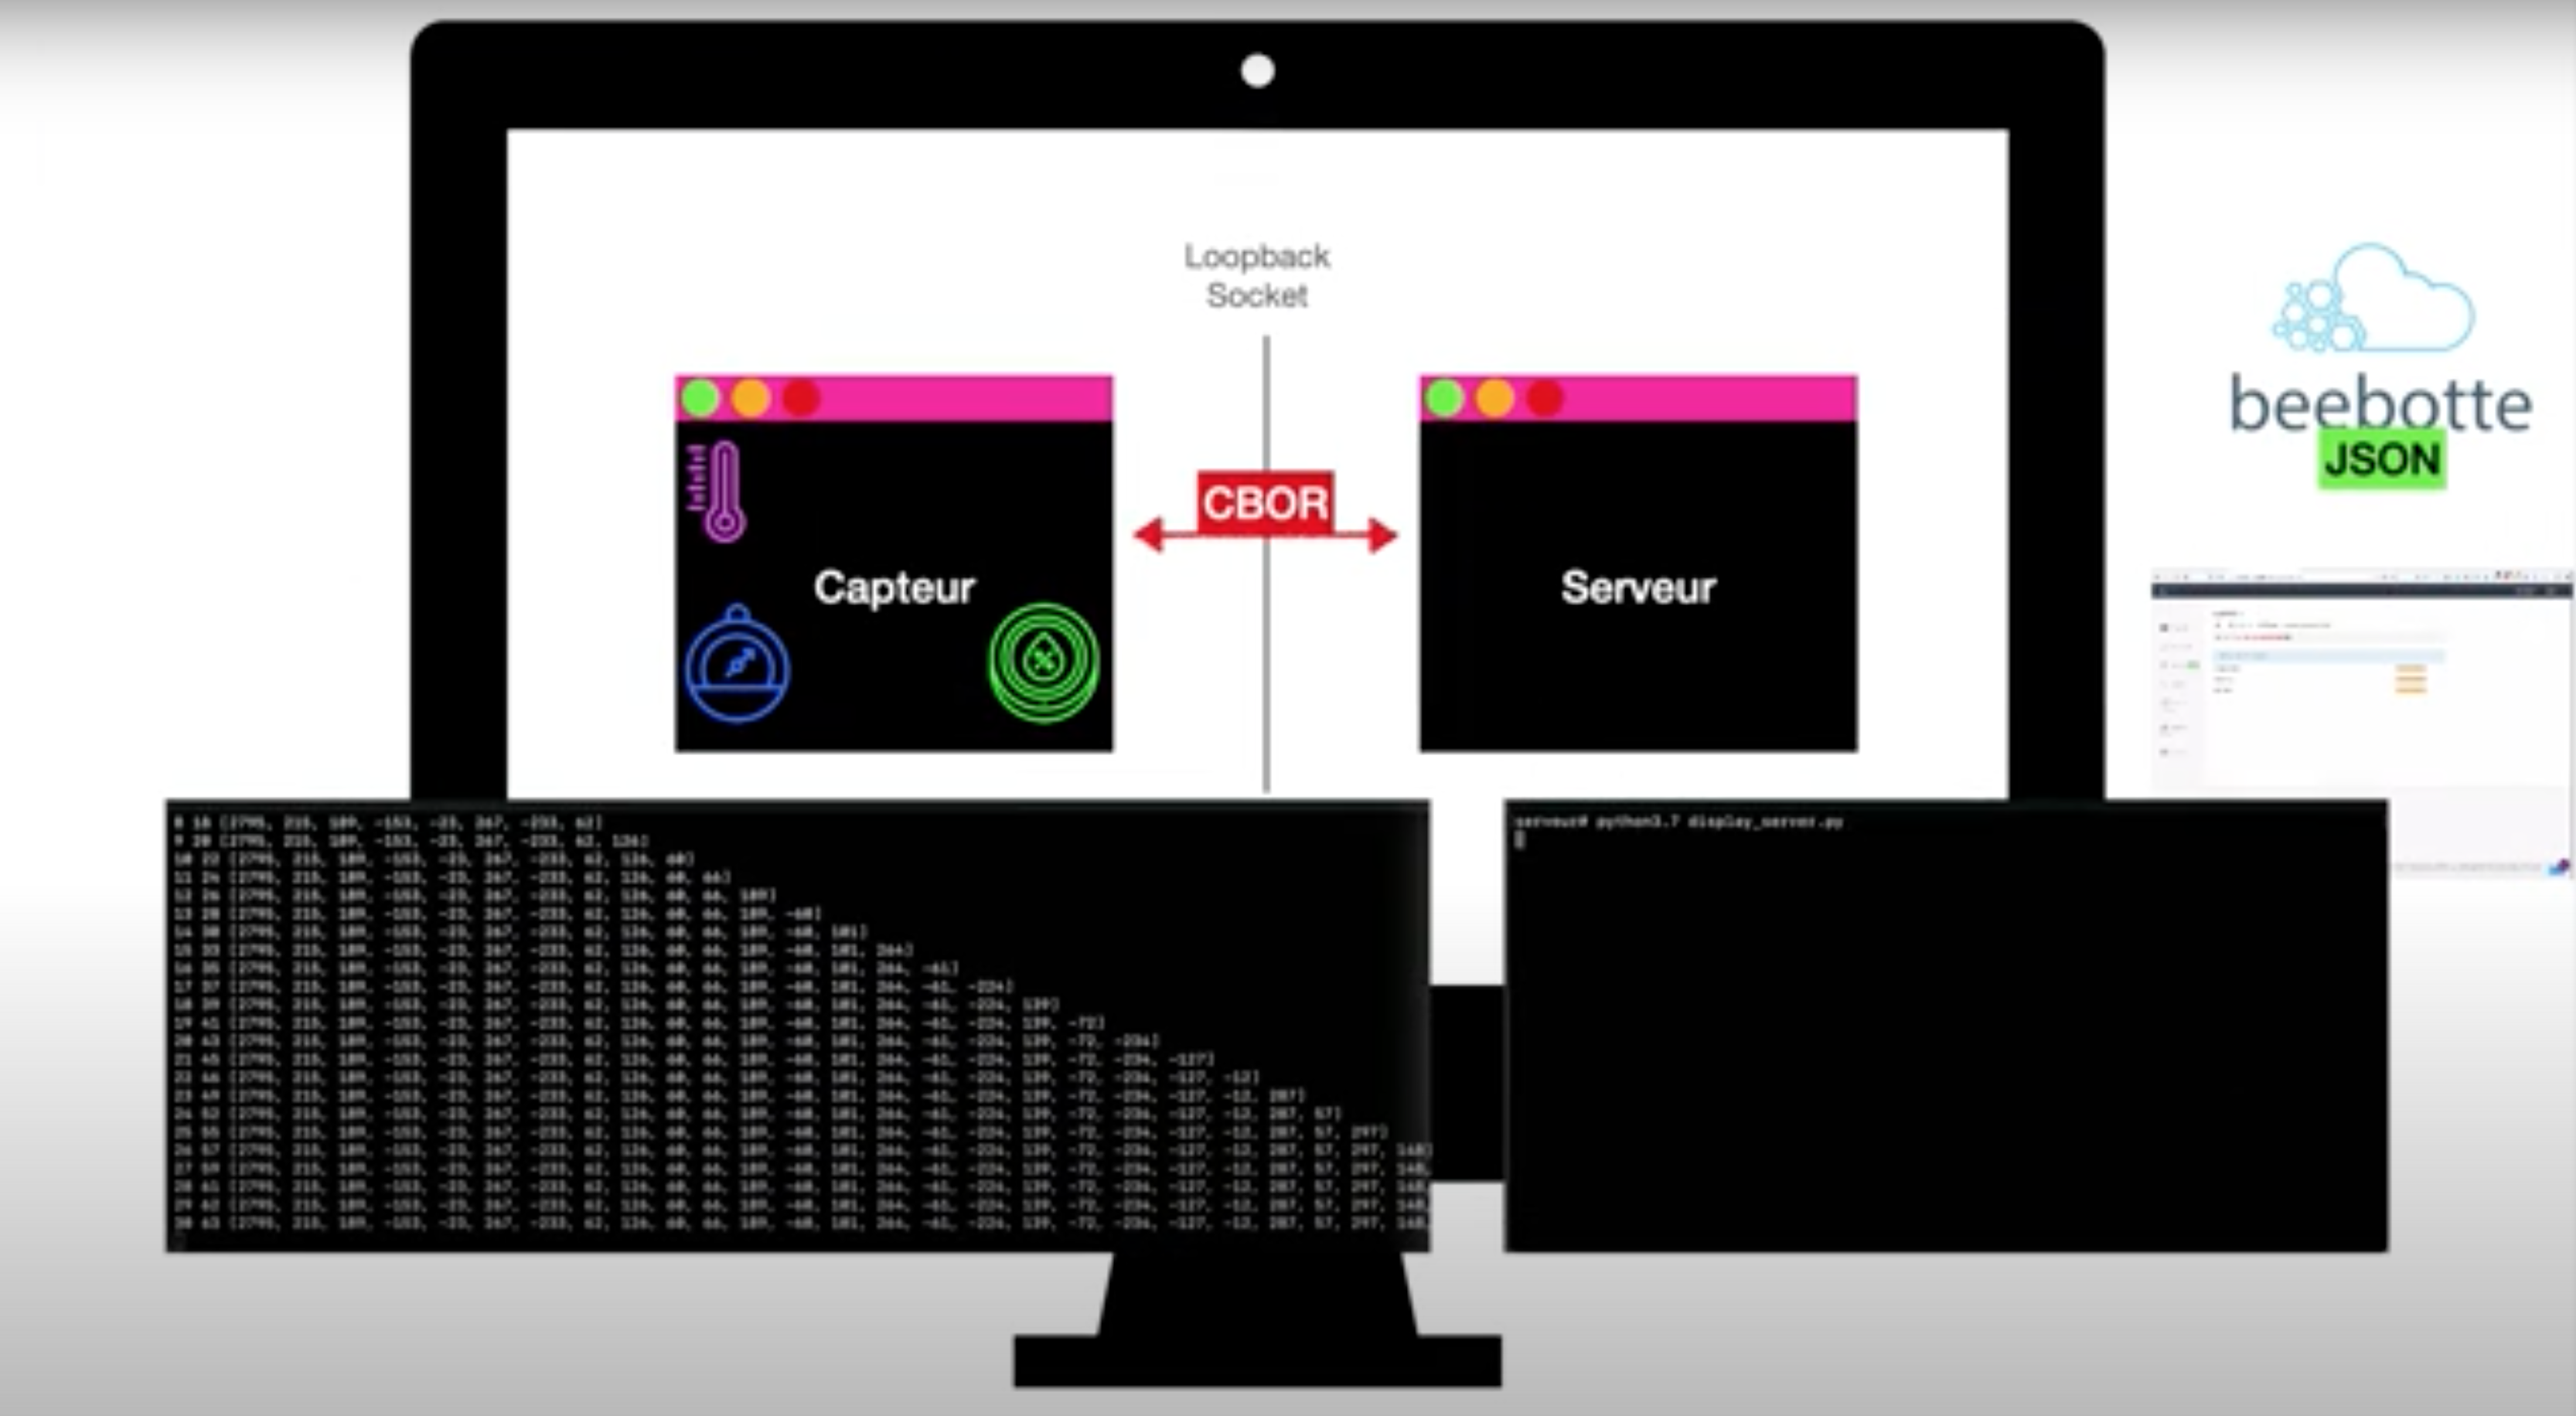
\includegraphics[width=1\columnwidth]{Pictures/Capture40.png}}
\caption{Architecture Client/Serveur}
\label{fig-client-serveur}
\end{figure}

\section{\Index{Beebotte}}

Il existe plusieurs sites qui permettent de le faire. Nous allons utiliser \url{https://beebotte.com}, mais ce que nous allons présenter peut très bien s'appliquer à d'autres sites.

\subsection{Configuration}

\begin{wrapfigure}{r}{3cm}

\includegraphics[width=.2\columnwidth]{Pictures/beebotte.png}
\end{wrapfigure}

La première étape consiste à créer un compte en cliquant sur \textit{Sign Up} sur la page de garde et en remplissant un formulaire classique avec votre login, adresse de courrier électronique et mot de passe. Une fois le compte validé, le service est accessible.

Le compte nous permet de nous authentifier pour gérer les données sur le site, mais il faut également disposer d’autorisation pour pouvoir y déposer des données via l’\Index{API REST}. Pour cela, il faut se rendre sur la page \textit{Account Setting} puis l’onglet \textit{Access Management}. Cette page (cf. figure~\vref{fig-bb-key}) donne une clé et un secret pour gérer l’ensemble des données sur le site. 

\begin{figure}[tbp]
\centerline{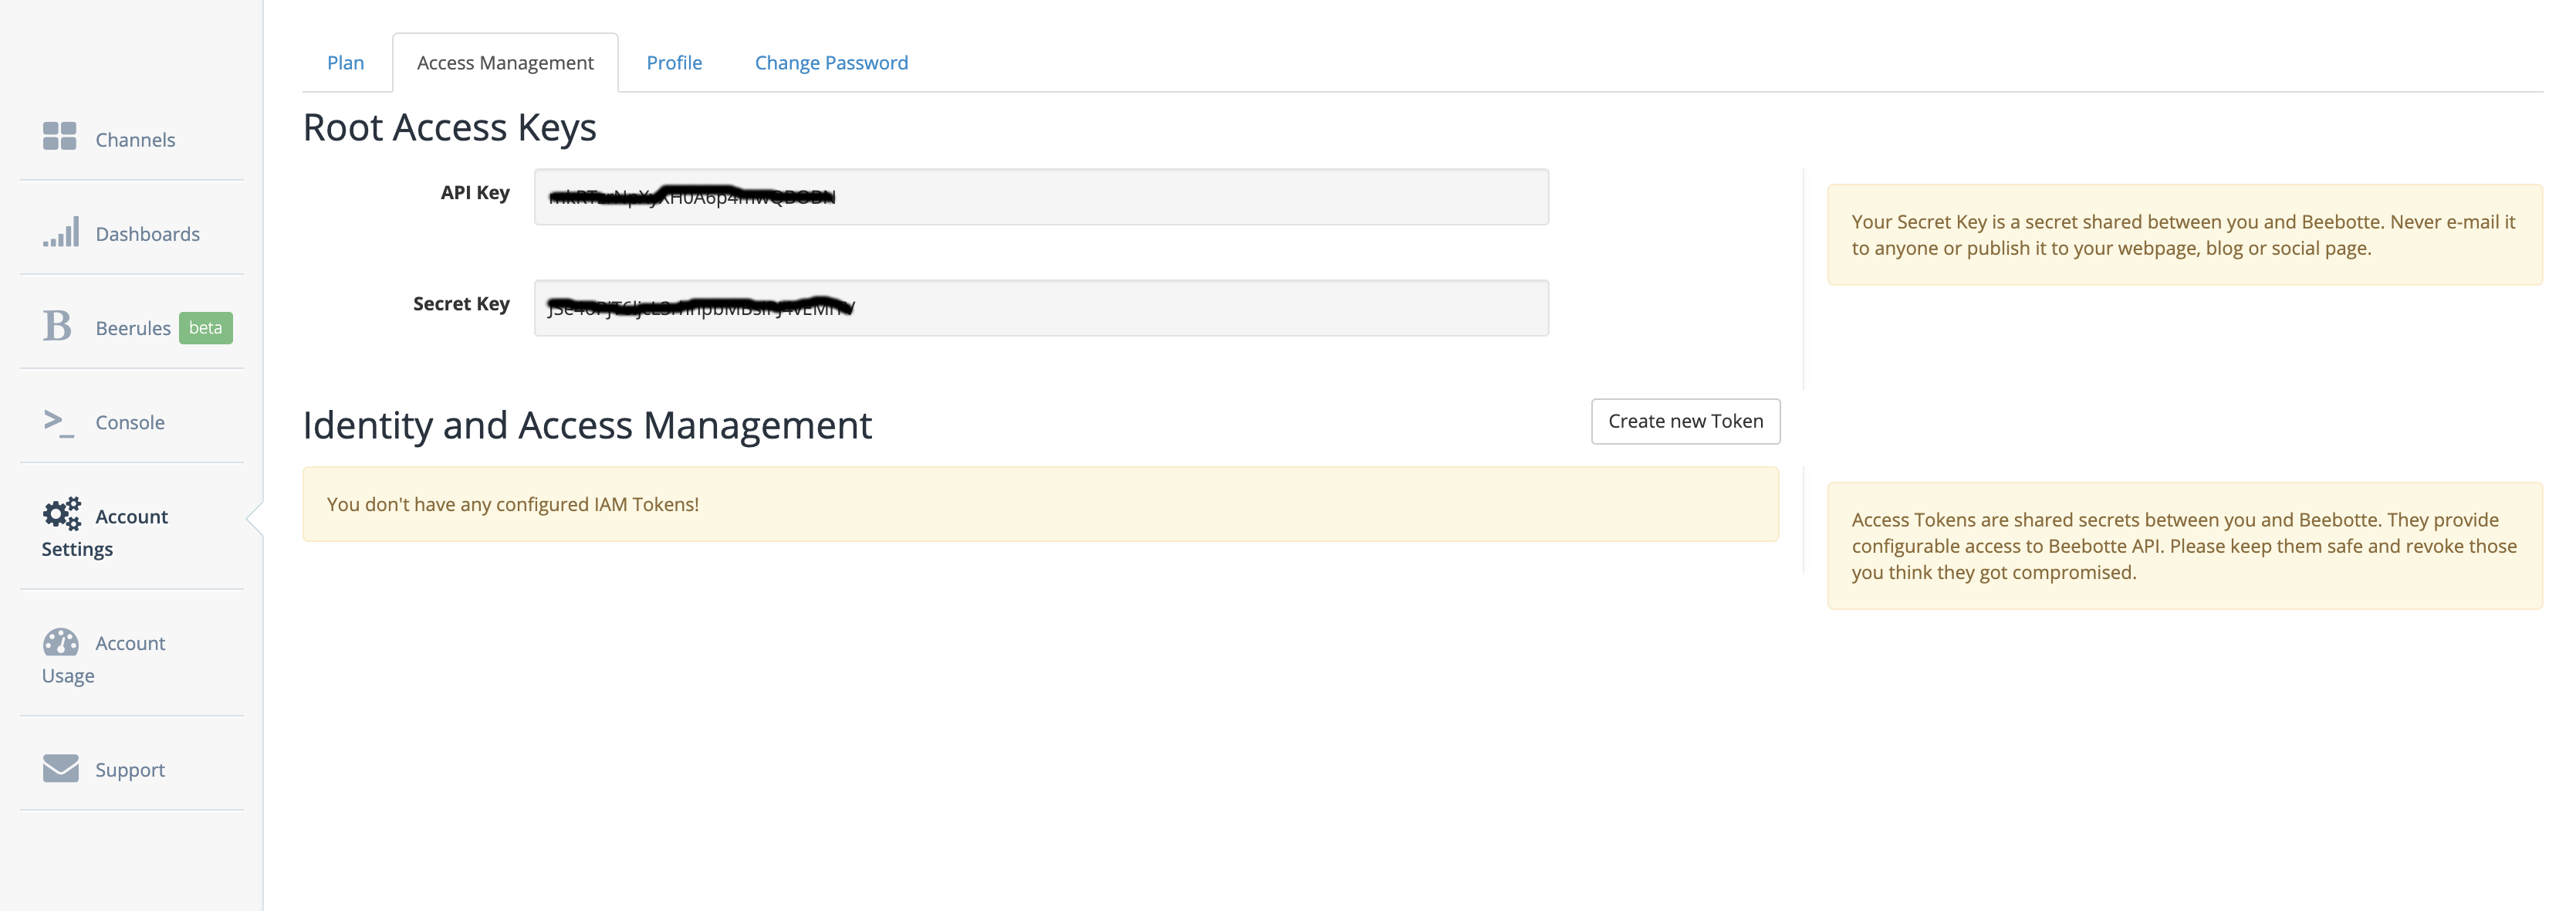
\includegraphics[width=1\columnwidth]{Pictures/bb_root_token.png}}
\caption{Clé et secret pour l'authentification}
\label{fig-bb-key}
\end{figure}


Notez ces valeurs et stockez les dans un fichier \pprog{config\_bbt.py} qui a cet aspect (vos valeurs sont forcément différentes) :

\pythonlst{config_bbt.py}




Nous allons maintenant créer un canal (/textit{channel}) dans lequel nous allons définir les objets correspondant aux capteurs. En Cliquant sur \textit {Channels} puis \textit{Create New}, la page représentée figure~\vref{fig-new-channel} apparaît. 

Il faut donner un nom au channel (\textit{capteurs} dans l'exemple), cocher la case \textit{public} et créer trois ressources pour les trois valeurs qui nous intéressent (\textit{temperature}, \textit{humidity}, \textit{presure}) et faire correspondre les unités.



\subsection{Enregistrement des ressources}

Le programme \pprog{display\_server.py} permet de correspondre avec Beebotte via son API REST. Il commence par l'importation des modules nécessaires~:

\pythonlst[firstline=1,lastline=8, firstnumber=1]{display\_server.py}


\begin{itemize}
    \item ligne 4, le module Python \texttt{beebotte}  est disponible pour simplifier la manipulation des données\footnote{S'il n'était pas présent sur votre ordinateur, vous devriez l'installer avec la commande \texttt{pip3 install beebotte}.}.
    \item ligne 5, le module \texttt{contient} la clé et le secret nécessaire à la connexion obtenu précédemment.
    
\end{itemize}



\pythonnxt[firstline=9,lastline=11, firstnumber=9]{display\_server.py}

\begin{itemize}
    \item ligne 10 et 11 permette d'ouvrir la socket pour communiquer avec les capteurs.
\end{itemize}

\pythonnxt[firstline=12,lastline=14, firstnumber=12]{display\_server.py}


\begin{itemize}
    \item ligne 13 une instance permettant la connexion avec les serveurs de Beebotte est définie grâce à la fonction \pfunction{beebotte}{BBT}. Les paramètres de connexion provenant du module \texttt{config\_bbt} sont pris en compte. 
\end{itemize}


\pythonnxt[firstline=41,lastline=45, firstnumber=41]{display\_server.py}

Dans le programme principal, un boucle sans fin attend la série temporelle codée en CBOR venant du capteur (ligne 42), les transforme tableau Python (ligne 44) et appelle la fonction \texttt{to\_btt} en précisant\:
\begin{itemize}
    \item le canal et la ressource qui ont été définie précédemment sur Beebotte~;
    \item la série temporelle
    \item la précision pour transformer ces entiers en flottant.
\end{itemize}
.  

\pythonnxt[firstline=15,lastline=38, firstnumber=15]{display\_server.py}

La fonction \texttt{to\_bbt} fait l’essentiel du travail de transformation. Elle prend en argument :

\begin{itemize}
    \item le nom du canal créé sur Beebotte. Dans notre cas, ce sera \texttt{capteurs} ;
    \item le nom de l’objet dans ce canal que nous avons également créé sur le site web. Dans notre cas, ce sera \texttt{humidity} ;
    \item le tableau python des mesures codées en delta ;
    \item le facteur multiplicatif, c’est-à-dire la précision. Ici, il faudra diviser par 100 ;
    \item la période entre deux mesures ; cela nous permettra de calculer l’instant de la mesure. Par défaut, la période est de 10 secondes ;
    \item le temps de réception du message pour dater les échantillons. S’il n’est pas spécifié, le temps courant est pris.

\end{itemize}

       \vspace{1em}

Cette fonction transforme le tableau Python suivant :
\begin{termc}[backgroundcolor=\color{palerod}, language=json, basicstyle=\ttfamily\small, escapechar=#]
[3311, 124, -144, -188, -94, 289, -1, -72, 1 ...
\end{termc}

en un tableau de dictionnaire :

\begin{termc}[backgroundcolor=\color{palerod}, language=json, basicstyle=\ttfamily\small, escapechar=#]
[{'data': 33.11, 'resource': 'humidity', 'ts': 1596730115000.0},
 {'data': 34.35, 'resource': 'humidity', 'ts': 1596730125000.0},
 {'data': 32.91, 'resource': 'humidity', 'ts': 1596730135000.0},
 {'data': 31.03, 'resource': 'humidity', 'ts': 1596730145000.0},
 ...
\end{termc}

       \vspace{1em}

Chaque dictionnaire contient trois éléments imposés par beebotte :

\begin{itemize}
\item le nom de la ressource (\texttt{resource}) telle qu’elle a été définie sur l’interface pour le canal ;
\item la valeur associée pour cette ressource (\texttt{data}) ;
\item l’instant à laquelle cette mesure à été faite\texttt{ (}ts). Le temps est représenté suivant le format \Index{Epoch} qui compte le nombre de secondes depuis le 1er Janvier 1970\footnote{voir \url{https://www.epochconverter.com/} pour les conversions.}.
\end{itemize}

       \vspace{1em}

Le calcul du timestamp (\textt{ts}) est l’opération la plus complexe de cette fonction mais les module \texttt{time} et \texttt{datetime} facilitent le calcul. 
Si l'argument \texttt{epoch} a été fourni lors de l'appel, la fonction prend cette valeur, sinon le calcule ligne 23. La fonction \pfunction{datetime}{now} retourne la date et l'heure courante, qui est transformé en un tuple grâce à la fonction \pfunction{datetime}{timetuple}. A partir de ce dernier, la fonction \pfunction{time}{maketime} le converti en epoch. 



Ligne 25, l'epoch à laquelle la première mesure du tableau a été faite est calculé en prenant le temps actuel (cela suppose que l’on néglige le temps de traitement et de transmission) auquel on retranche la durée de la capture, c’est-à-dire comme le nombre d’éléments du tableau multiplié par l’intervalle entre chaque mesure (\texttt{period}). 

Ligne 32 à 34 la structure attendue par Beebotte est construite. le résultat est envoyé, ligne 38, grâce à la fonction \pfunction{beebotte}{writeBulk} qui permet d'envoyer un ensemble de valeurs.

       \vspace{1em}

On peut vérifier que Beebotte a reçu des données en visualisant le canal capteurs sur l’interface Web. On peut voir sur la  figure~\vref{fig-bb-mesure} que seule la ressource \texttt{humidity} a reçu des données. L’interface affiche la dernière valeur reçue et la date de réception.

\begin{figure}[tbp]
\centerline{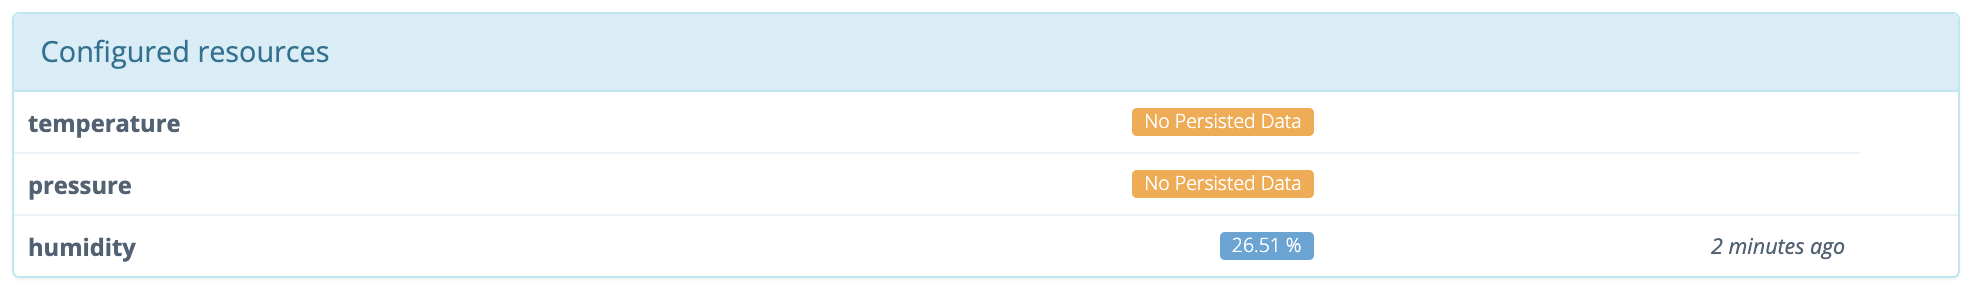
\includegraphics[width=1\columnwidth]{Pictures/bb_mesures.png}}
\caption{État des ressources}
\label{fig-bb-mesure}
\end{figure}

\subsection{Visualisation des ressources}

